\documentclass[12pt]{article}
\usepackage{fullpage}
\usepackage{graphicx}
\usepackage{subfigure}
\usepackage{amsmath}
\usepackage{amsfonts}
\usepackage{amssymb}
\usepackage{amsbsy}
\usepackage{setspace}
\usepackage{fullpage}
\usepackage{wrapfig}
\usepackage{cite}
\usepackage{float}
\usepackage{algorithm, algpseudocode}

\usepackage[skip=2pt,font=footnotesize]{caption}

\begin{document}
\begin{center}
 \LARGE\textbf{Coupled Growth and Fluid Medium for Time-Lapse Modeling}
\end{center}

\tableofcontents
%\newpage
\clearpage
% new commands for the CHT paper defined by Fanlong are listed at the very bottom

\renewcommand{\url}[1]{}% ******** Remove URL's from bibtex entries ********
\newcommand{\citeCount}[1]{}% for citation counts papers for WDH citations
% 
\newtheorem{theorem}{Theorem}
\newtheorem{Algorithm}{Algorithm}
\newtheorem{procedure}{Procedure}
\newtheorem{lemma}{Lemma}
\newtheorem{definition}{Definition}
\newtheorem{proposition}{Proposition}
\newtheorem{assumption}{Assumption}
\newtheorem{condition}{Condition}
% \newtheorem{AMPInterfaceCondition}{AMP Interface Condition}
\newtheorem{AMPInterfaceCondition}{Interface Condition}
\newtheorem{modelProblem}{Model Problem}
\newtheorem{travelingWave}{Traveling Wave Exact Solution}

\newtheorem*{algorithmAMP}{AMP Algorithm (added-mass partitioned) }
\newtheorem*{algorithmTP}{TP Algorithm (traditional partitioned)}

\newtheorem*{ModelProblemIA}{Model Problem MP-IA}
\newtheorem*{ModelProblemVA}{Model Problem MP-VA}
\newtheorem*{ModelProblemVE}{Model Problem MP-VE}

\newcommand{\dx}{\Delta x}
\newcommand{\dy}{\Delta y}
\newcommand{\dt}{\Delta t}


% \newcommand{\kappaR}{{\rhoR\cR^2}}

\newcommand{\Dp}{D_{+}}
\newcommand{\Dm}{D_{-}}
\newcommand{\Dpx}{D_{+x}}
\newcommand{\Dmx}{D_{-x}}
\newcommand{\Dpy}{D_{+y}}
\newcommand{\Dmy}{D_{-y}}

\newcommand{\erf}{\operatorname{erf}}

    
\newcommand{\bogus}[1]{{}}

% -----Bill's common definitions-----

\newcommand{\av}{\mathbf{ a}}
\newcommand{\bv}{\mathbf{ b}}
\newcommand{\cv}{\mathbf{ c}}
\newcommand{\dv}{\mathbf{ d}}
\newcommand{\ev}{\mathbf{ e}}
\newcommand{\fv}{\mathbf{ f}}
\newcommand{\gv}{\mathbf{ g}}
\newcommand{\hv}{\mathbf{ h}}
\newcommand{\iv}{\mathbf{ i}}
\newcommand{\jv}{\mathbf{ j}}
\newcommand{\kv}{\mathbf{ k}}
\newcommand{\lv}{\mathbf{ l}}
\newcommand{\mv}{\mathbf{ m}}
\newcommand{\nv}{\mathbf{ n}}
\newcommand{\ov}{\mathbf{ o}}
\newcommand{\pv}{\mathbf{ p}}
\newcommand{\qv}{\mathbf{ q}}
\newcommand{\rv}{\mathbf{ r}}
\newcommand{\sv}{\mathbf{ s}}
\newcommand{\tv}{\mathbf{ t}}
\newcommand{\uv}{\mathbf{ u}}
\newcommand{\vv}{\mathbf{ v}}
\newcommand{\wv}{\mathbf{ w}}
\newcommand{\xv}{\mathbf{ x}}
\newcommand{\yv}{\mathbf{ y}}
\newcommand{\zv}{\mathbf{ z}}
% 
\newcommand{\Av}{\mathbf{ A}}
\newcommand{\Bv}{\mathbf{ B}}
\newcommand{\Cv}{\mathbf{ C}}
\newcommand{\Dv}{\mathbf{ D}}
\newcommand{\Ev}{\mathbf{ E}}
\newcommand{\Fv}{\mathbf{ F}}
\newcommand{\Gv}{\mathbf{ G}}
\newcommand{\Hv}{\mathbf{ H}}
\newcommand{\Iv}{\mathbf{ I}}
\newcommand{\Jv}{\mathbf{ J}}
\newcommand{\Kv}{\mathbf{ K}}
\newcommand{\Lv}{\mathbf{ L}}
\newcommand{\Mv}{\mathbf{ M}}
\newcommand{\Nv}{\mathbf{ N}}
\newcommand{\Ov}{\mathbf{ O}}
\newcommand{\Pv}{\mathbf{ P}}
\newcommand{\Qv}{\mathbf{ Q}}
\newcommand{\Rv}{\mathbf{ R}}
\newcommand{\Sv}{\mathbf{ S}}
\newcommand{\Tv}{\mathbf{ T}}
\newcommand{\Uv}{\mathbf{ U}}
\newcommand{\Vv}{\mathbf{ V}}
\newcommand{\Wv}{\mathbf{ W}}
\newcommand{\Xv}{\mathbf{ X}}
\newcommand{\Yv}{\mathbf{ Y}}
\newcommand{\Zv}{\mathbf{ Z}}

\newcommand{\collon}{:}  % note \colon already defined by someone.
\newcommand{\ff}{\tt}

% \newcommand{\lt}{{<}}
% \newcommand{\grad}{\nabla}
% \newcommand{\comma}{~~~,~~}
% \newcommand{\calo}{{\cal O}}

\newcommand{\half}{{1\over2}}

\newcommand{\Real}{{\mathbb R}}
\newcommand{\Complex}{{\mathbb C}}

\newcommand{\zerov}{\mathbf{0}}


\newcommand{\Ac}{{\mathcal A}}
\newcommand{\Bc}{{\mathcal B}}
\newcommand{\Cc}{{\mathcal C}}
\newcommand{\Dc}{{\mathcal D}}
\newcommand{\Ec}{{\mathcal E}}
\newcommand{\Gs}{{\mathcal G}}
\newcommand{\Ic}{{\mathcal I}}
\newcommand{\Rc}{{\mathcal R}}
\newcommand{\Gc}{{\mathcal G}}
\newcommand{\Lc}{{\mathcal L}}
\newcommand{\Nc}{{\mathcal N}}
\newcommand{\Oc}{{\mathcal O}}
\newcommand{\Pc}{{\mathcal P}}
\newcommand{\Qc}{{\mathcal Q}}
\newcommand{\Tc}{{\mathcal T}}



\newcommand{\deltav}{\boldsymbol{\delta}}
\newcommand{\omegav}{\boldsymbol{\omega}}
\newcommand{\tauv}{\boldsymbol{\tau}}
\newcommand{\phiv}{\boldsymbol{\phi}}
\newcommand{\psiv}{\boldsymbol{\psi}}
\newcommand{\sigmav}{\boldsymbol{\sigma}}
\newcommand{\chiv}{\boldsymbol{\chi}}


\newcommand{\grad}{\nabla}

% \newcommand{\tableFont}{\scriptsize}
\newcommand{\tableFont}{\footnotesize}
\newcommand{\tableFontSize}{\tableFont}
\newcommand{\num}[2]{#1e#2} % Use this macro to define the format of the numbers in the table
\newcommand{\errFormat}[1]{$e_{#1}$} % form of error label in tables
\newcommand{\eem}{e^{(j)}}
\newcommand{\rateLabel}{rate}

\clearpage
\newcommand{\dtau}{\delta_\tau}
\newcommand{\Gb}{G}


\newcommand{\As}{\bar{A}}
\newcommand{\Ks}{\bar{K}}
% \newcommand{\Fs}{\bar{F}}

\newcommand{\rhos}{\bar{\rho}}
\newcommand{\cp}{\bar{c}_p}
\newcommand{\cs}{\bar{c}_s}
\newcommand{\kappas}{{\rhos\cs^2}}
\newcommand{\zs}{{\bar {z}}}  % solid impedance based on c_p
\newcommand{\zp}{z_p}  % solid impedance based on c_s
\newcommand{\us}{\bar{u}}
\newcommand{\qs}{\bar{q}}
\newcommand{\vs}{\bar{v}}
\newcommand{\sigmas}{\bar{\sigma}}
\newcommand{\xs}{\bar{x}}
\newcommand{\xsv}{\bar{\xv}}
\newcommand{\gsv}{\bar{\gv}}
\newcommand{\rsv}{\bar{\rv}}
\newcommand{\rs}{\bar{r}}
\newcommand{\xf}{{x}}
\newcommand{\dxs}{\Delta{\bar x}}
\newcommand{\dxf}{{\Delta x}}
\newcommand{\Ns}{\bar{N}}
\newcommand{\Nf}{{N}}
\newcommand{\zf}{z_f}

\newcommand{\usv}{\bar{\uv}}
\newcommand{\vsv}{\bar{\vv}}
\newcommand{\wsv}{\bar{\wv}}

\newcommand{\ush}{\hat{\us}}
\newcommand{\usvh}{\hat{\usv}}
\newcommand{\vvh}{\hat{\vv}}
\newcommand{\vh}{\hat{v}}
\newcommand{\ph}{\hat{p}}

\newcommand{\nsv}{\bar{\nv}}
\newcommand{\vvs}{\bar{\vv}}
\newcommand{\uvs}{\bar{\uv}}
\newcommand{\xvs}{\bar{\xv}}
\newcommand{\sigmavs}{\bar{\sigmav}}
\newcommand{\sigmasv}{\bar{\sigmav}}
\newcommand{\fsv}{\bar{\fv}}
\newcommand{\qsv}{\bar{\qv}}

\newcommand{\qsvp}{\qsv^p}
\newcommand{\qsvI}{\qsv^I}
\newcommand{\qvI}{\qv^I}

\newcommand{\vvI}{\vv^I}
\newcommand{\tauvI}{\tauv^I}
\newcommand{\vvIf}{\vv^f}
\newcommand{\tauvIf}{\tauv^f}
% \newcommand{\vvIf}{\vv^{I,f}}
\newcommand{\sigmavI}{\sigmav^I}
\newcommand{\vsvIs}{\vsv^s}
\newcommand{\sigmavIs}{\sigmav^s}

\newcommand{\dvel}{{\delta_v}}
\newcommand{\vDot}{\dot{v}}
\newcommand{\vsDot}{\dot{\vs}}
\newcommand{\vvDot}{\dot{\vv}}
\newcommand{\vsvDot}{\dot{\vsv}}

% \newcommand{\rb}{r_b} % a point on the body surface

% \newcommand{\amp}{{\mathcal{A}}}
\newcommand{\amp}{A}


% \newcommand{\Energy}{\mathcal{E}}% Energy of the fluid
% \newcommand{\Area}{\mathcal{A}_b}
% \newcommand{\Area}{A_b}
% \newcommand{\width}{\mathcal{W}}
% \newcommand{\width}{w_b}


\newcommand{\charSpeed}{s}% Char. speed
\newcommand{\charVar}{\chi}% Char. variable


\newcommand{\largess}{\sffamily\large}
\newcommand{\Largess}{\sffamily\Large}
\newcommand{\bfss}{\sffamily\bfseries}
\newcommand{\smallss}{\sffamily\small}
\newcommand{\normalss}{\sffamily}
\newcommand{\scriptsizess}{\sffamily\scriptsize}

\newcommand{\hs}{\bar{h}}
% \newcommand{\Hs}{H_s}
\newcommand{\Hs}{\bar{H}}

\newcommand{\kxHat}{\hat{k}_x}
\newcommand{\kyHat}{\hat{k}_y}
\newcommand{\omegaHat}{\hat{\omega}}
\newcommand{\aHat}{\hat{a}}
\newcommand{\bHat}{\hat{b}}

\newcommand{\aTilde}{\tilde{a}}
\newcommand{\bTilde}{\tilde{b}}

\newcommand{\qsHat}{\hat{\qs}}
\newcommand{\phase}{x_0}
\newcommand{\phaset}{t_0}

\newcommand{\as}{\bar{a}}
\newcommand{\bs}{\bar{b}}
\newcommand{\ds}{\bar{d}}
\newcommand{\asHat}{\hat{\as}}
\newcommand{\bsHat}{\hat{\bs}}
\newcommand{\dsHat}{\hat{\ds}}

\newcommand{\dHat}{\hat{d}}
\newcommand{\pHat}{\hat{p}}
\newcommand{\qHat}{\hat{q}}
\newcommand{\vHat}{\hat{v}}
\newcommand{\vvHat}{\hat{\vv}}
\newcommand{\vsHat}{\hat{\vs}}
\newcommand{\sigmaHat}{\hat{\sigma}}
\newcommand{\sigmasHat}{\hat{\sigmas}}

\newcommand{\lambdas}{\bar{\lambda}}% solid Lame' parameter
\newcommand{\mus}{\bar{\mu}}% solid Lame' parameter

\newcommand{\OmegaF}{\Omega^F}% fluid domain
\newcommand{\OmegaS}{\Omega^S}% solid domain

\newcommand{\OmegaFh}{\Omega^F_h}% fluid domain
\newcommand{\OmegaSh}{\Omega^S_h}% solid domain

\newcommand{\GammaI}{\Gamma}% Fluid-Solid Interface
\newcommand{\Gammas}{\bar{\Gamma}}% Fluid-Solid Interface, reference space
\newcommand{\GammaIh}{\Gamma_h}% Fluid-Solid Interface

\renewcommand{\zp}{\bar{z}_p}
\renewcommand{\zs}{\bar{z}_s}
\newcommand{\zb}{\bar{z}}
\newcommand{\Lt}{\tilde{L}}

\newcommand{\MR}{M_r}% added mass ratio
\newcommand{\Mr}{\mathcal{M}}% another added mass ratio

\newcommand{\phis}{\phi_s}
\newcommand{\phib}{\phi_b}
% \newcommand{\phit}{\tilde{\phi}}
% \newcommand{\phit}{\phi_<}

\newcommand{\phim}{\phi_-}
\newcommand{\phip}{\phi_+}


\newcommand{\lambday}{\lambda}% 
\newcommand{\lambdax}{\lambda_x}% 

\newcommand{\cb}{\bar{c}}
\newcommand{\kk}{k_x} % wave number of 2d analysis
\newcommand{\kx}{k_x} % wave number of 2d analysis
\newcommand{\ax}{\alpha \amp^{m+1}}
\newcommand{\thetaj}{\theta} % Jeff's theta


% Predicted states:
% \newcommand{\vvp}{\vv^p}
% \newcommand{\vp}{v^p}
\newcommand{\sigmavp}{\sigmav^p}
\newcommand{\sigmap}{\sigma^p}
\newcommand{\tauvp}{\tauv^p}
\newcommand{\taup}{\tau^p}
\newcommand{\vsvp}{\vsv^p}
\newcommand{\vsp}{\vs^p}
\newcommand{\sigmasvp}{\sigmasv^p}
\newcommand{\sigmasp}{\sigmas^p}


\newcommand{\Ck}{C_k}
\newcommand{\Sk}{S_k}
\newcommand{\Ca}{C_\alpha}
\newcommand{\Sa}{S_\alpha}

\newcommand{\Sas}{S_a}
\newcommand{\Cas}{C_a}
\newcommand{\Sbs}{S_b}
\newcommand{\Cbs}{C_b}

\newcommand{\dsf}{\delta}


\newcommand{\expkw}{e^{i(k x -\omega t)}}
% \newcommand{\ampe}{\Ac_0}% amplitude of exact solution
\newcommand{\ampe}{{\bar u_{{\rm max}}}}


% \newcommand{\nus}{\bar\nu}
\newcommand{\betas}{\bar\beta}
% \newcommand{\ly}{\ell_y}
% \newcommand{\lx}{\ell_x}
% \newcommand{\ly}{\beta_y}
% \newcommand{\lx}{\beta_x}
% \newcommand{\ly}{\alpha_y}
% \newcommand{\lx}{\alpha_x}
\newcommand{\ly}{\lambda_y}
\newcommand{\lx}{\lambda_x}
% \newcommand{\ly}{\gamma_y}
% \newcommand{\lx}{\gamma_x}

\newcommand{\tanv}{\tv}% tangent 
\newcommand{\blue}{\color{blue}}
\newcommand{\red}{\color{red}}
\newcommand{\green}{\color{green}}

\newcommand{\strutt}{\rule{0pt}{10pt}}% strutt to make table height bigger
\newcommand{\tr}{\text{tr}}% trace


\newcommand{\nd}{{n_d}} % number of space dims


% JCP \newcommand{\Fig}{Fig.} % refer to figures this way
\newcommand{\Fig}{Figure} % refer to figures this way
\newcommand{\wvs}{\bar{\wv}}% solid `w
% \newcommand{\wsv}{\bar{\wv}}% solid `w

% \newcommand{\as}{c_p}% solid compression wave speed 
% \newcommand{\azs}{c_p}% solid compression wave speed 

\newcommand{\Pbar}{\bar{P}}
\newcommand{\Fbar}{\bar{F}}
\newcommand{\Ps}{\Pbar}
\newcommand{\Fs}{\Fbar}
% \newcommand{\fs}{{\bar{f}}


% \newcommand\Omegaf{{\Omega}}
\newcommand\Omegas{{\bar\Omega}}
% \newcommand\Gammas{{\bar\Gamma}}
% \newcommand\ps{{\bar P}}
% \newcommand\ks{{\bar K}}
% \newcommand\js{{\bar J}}
% \newcommand\Ss{{\bar S}}
% \newcommand\es{{\bar E}}
% \newcommand\Cs{{\tilde E}}
% \newcommand\CC{{\bar C}}
% \newcommand\stressStrain{{\cal S}}
% 
% \newcommand{\Js}{\bar{J}}


\newcommand\Ts{{\bar T}}
%\newcommand\tsv{{\bar\tv}}
\newcommand\ns{{\bar n}}
\newcommand\ts{{\bar\tau}}
%\newcommand\ts{{\bar t}}
% \newcommand\leftv{{\bar\yv}}
% \newcommand\vvr{{\tilde\vv}}
% \newcommand\rotation{{R}}
% \newcommand\leftvr{{\tilde\yv}}
% \newcommand\vr{{\tilde v}}

%\newcommand\stress{{\bar s}}
%\newcommand\stressv{{\bar\sv}}
%\newcommand\stressvr{{\tilde\sv}}
%\newcommand\stressfv{{\sv}}
%\newcommand\stressf{{s}}
%\newcommand\stressr{{\tilde s}}
\newcommand\stress{{\bar w}}
\newcommand\stressv{{\bar\wv}}
\newcommand\stressvr{{\tilde\wv}}
\newcommand\stressfv{{\wv}}
\newcommand\stressf{{w}}
\newcommand\stressr{{\tilde w}}


% -- prime variables
\newcommand{\xp}{x'}
\newcommand{\vp}{v'}
\newcommand{\xsp}{\xs'}
\newcommand{\Pp}{P'}
\newcommand{\Tp}{T'}
\newcommand{\qvp}{\qv'}
\newcommand{\qpv}{\qvp}

% interface point:
\newcommand\Qs{{\bar Q}}
\newcommand\Qf{{Q}}
\newcommand{\interfacePoint}{\Qf}
\newcommand{\interfacePointSolid}{\Qs}% in solid ref frame

\newcommand{\Gep}{\Gc_{ep}} % elastic piston grid
\newcommand{\Gd}{\Gc_{\text{rd}}}% rotating disk grid
\newcommand{\Ge}{\Gc_{e}} % deforming ellipse

\newcommand\ths{{\bar\theta}}
\newcommand\usr{{\us_r}}
\newcommand\ust{{\us_\theta}}
\newcommand\psr{{\tilde P}}
\newcommand\Vr{{\bar V}}

\newcommand\Jg{J_g}
\newcommand\Jsg{\Js_g}

\newcommand{\timeScale}{t^*}

% tangent: 
\newcommand\tn{{t}}
\newcommand\tnv{{\mathbf{t}}}
\newcommand\tns{{\bar\tn}}
\newcommand\tnvs{{\bar\tnv}}
\renewcommand\tv{\tnv}
\newcommand\tsv{\tnvs}


\newcommand\bsolid{{\bar b}}

\newcommand{\shift}{E}% shift operator


% \newcommand{\omegav}{\boldsymbol{\omega}}
\newcommand{\cm}{{\rm cm}}
\newcommand{\mrb}{m_{b}}% mass of the body
% \newcommand{\xvcm}{\xv_{\rm cm}}% position of the center of mass
% \newcommand{\vvcm}{\vv_{\rm cm}}% velocity of the center of mass
% \newcommand{\avcm}{\av_{\rm cm}}% acceleration of the center of mass
% \newcommand{\dotxvcm}{\dot\xv_{\rm cm}}% position of the center of mass
% \newcommand{\dotvvcm}{\dot\vv_{\rm cm}}% velocity of the center of mass
\newcommand{\xcm}{x_b}% position of the center of mass
\newcommand{\vcm}{v_b}% position of the center of mass
\newcommand{\xb}{x_b}% position of the center of mass
\newcommand{\vb}{v_b}% position of the center of mass
\newcommand{\xvb}{\xv_b}% position of the center of mass
\newcommand{\vvb}{\vv_b}% position of the center of mass
\newcommand{\avb}{\av_b}% acceleration of the center of mass
\newcommand{\bvb}{\bv_b}% angular acceleration of the center of mass
\newcommand{\xvcm}{\xv_b}% position of the center of mass
\newcommand{\vvcm}{\vv_b}% velocity of the center of mass
\newcommand{\avcm}{\av_b}% acceleration of the center of mass
\newcommand{\dotxcm}{\dot{x}_b}% position of the center of mass
\newcommand{\dotrb}{\dot{r}_b}% position of the center of mass
\newcommand{\dotvcm}{\dot{v}_b}% position of the center of mass
\newcommand{\dotvb}{\dot{v}_b}% position of the center of mass
\newcommand{\dotxvcm}{\dot\xv_b}% position of the center of mass
\newcommand{\dotvvcm}{\dot\vv_b}% velocity of the center of mass


% \newcommand{\dtau}{\delta_\tau}
% \newcommand{\Gb}{G}

\newcommand{\OmegaMatrix}{W}
\newcommand{\Force}{\mathcal{F}}
\newcommand{\Forcev}{\boldsymbol{\Force}}
\newcommand{\Forcevtilde}{\widetilde{\Forcev}}
\newcommand{\Fvtilde}{\Forcevtilde}
\newcommand{\Torque}{\mathcal{T}}
\newcommand{\Torquev}{\boldsymbol{\Torque}}
\newcommand{\Torquevtilde}{\widetilde{\Torquev}}
\newcommand{\Gvtilde}{\Torquevtilde}
\newcommand{\Ma}{A_m}

\newcommand{\mass}{{m_b}}
\newcommand{\force}{\Force}

%Fanlong's new commands
\newcommand{\f}{\frac}
\newcommand{\p}{\partial}
\newcommand{\ka}{\kappa}
\newcommand{\Kc}{{\mathcal K}}
\newcommand{\Tb}{{\bar T}}
\newcommand{\Ub}{{\bar U}}
\newcommand{\Kb}{{\bar {\mathcal K}}}
\newcommand{\Db}{{\bar {\mathcal D}}}

\section{BACKGROUND AND MOTIVATION - 2 pages}

\subsection{Growth of Cells and Tissues - 0.5 page}
In the mechanical view, the most distinguishable feature of living matters is their ability to respond to environmental changes while common engineering materials cannot. Hard tissues increase their density and grow strong. One common example is that tennis players have a significantly dominant arm. While training increases the strength of bones, it is also the cause of chronic pain that many athletes suffer \cite{Kuhl6}. Soft tissues increase their volume and grow large. For instance, myocardial infarction could cause the infarcted ventricle to dilate in response to volume overload, attempting to maintain normal cardiac output. Meanwhile the pumping efficiency may be reduced, resulting in the medical condition called cardiac dilation \cite{Guccione}. Growth plays a key role in many biological and medical processes including the cardiovascular disease, tumor growth, restenosis, trauma healing, twisted bone growth and so on. The research in life science has revealed a lot of fundamental phenomenon, which greatly enrich our understanding to living matters yet are still far from being applied. Clinical researchers, on the other hand, adopt an observational and experimental strategy to explore treatments. However, the progress is relatively slow because of the lack of understanding of underlying physics. Microscopically, growth is the result of the reproduction and rearrangement of microstructures; Macroscopically, growth is the adaption of materials to the mechanical loading governed by certain laws. Therefore, people gradually come to realize that the growth of cells and tissues could not be understood with a single discipline alone. Instead, it requires the inputs from biology, mechanics, and mathematics communities.

\subsection{Review of Mathematical and Mechanical Growth Models - 1 page}
The contribution from the mechanics community to the understanding of the growth of living biological materials dates back to a hundred years ago. Thompson \cite{Thompson} and Huxley \cite{Huxley} brought up the idea of organism-level morphological view where growth is characterized as a change in form. In the recent half century, a lot of breakthroughs have been made from the research on the mechanical impact on the biological materials. Early works include the growth velocity field representation (GVFR), which includes the use of path lines and streamlines \cite{Truesdell}. Applications of the GVFR have been reported in \cite{Erickson, Erickson2, Richards}. Despite of the simplicity, GVFR is criticized of lacking most of essential ingredients that constitute a theory of material behavior \cite{Cowin}.

Another approach is the multi-constituent open systems based on the theory of mixtures \cite{Bowen, Rajagopal}. This approach models solids and fluids as combinations of diverse constituents. It is useful for modeling evolving contributions of the different solid constituents that comprise a tissue or cell and influence its growth. The resulting equations are usually complicated. For instance Humphrey and Rajagopal \cite{Humphrey} suggested that full mixture equations for mass balance (including reaction-diffusion effects of vasoactive, mitogenic, synthetic, proteolytic and inflammatory molecules) be used in combination with classical equations for linear momentum balance written in terms of rule-of-mixture relations for the stress response.

Different from the mathematical biologists cited above, modern continuum mechanical community treats the growth as a change in mass without ignoring the related change in form \cite{Ambrosi}. The key problem is how to translate the change of mass into non-uniform changes in form. Progress was made in hard tissues first because they are easier than soft tissues for three reasons, as put by Menzel and Kuhl in \cite{Menzel}: first, since they do not undergo large deformations in vivo, a linear kinematic characterization is sufficiently accurate; second, although they are multiphase materials consisting of solid and fluid constituents, for most technical applications, a single phase characterization in terms of the solid constituent alone represents their behavior sufficiently well; third, since they are relatively easy to preserve, and their ex vivo response closely matches their in vivo behavior, which make them relatively easy to test. For instance, Cowin's work in \cite{Cowin} shows that in case of small deformation and rotation, the problem that the mapping between the reference configuration and the spatial configuration is not ``onto'' can be avoided because the two configurations can be considered as identical. A lot of insights are gained from the studies on the growth of hard tissues including the mechanism of how astronauts lose bones in space \cite{Kuhl2}, the reason why hip replacement and repair induce a local loss of bone density \cite{Ambrosi}, the relationship between osteoporosis and the local bone loss \cite{Pang} and so on.

The growth of soft tissues is much more difficult for the exactly the opposite reasons: they typically undergo large deformations and their accurate characterization requires a finite kinematic approach \cite{Rodriguez}; their multi-phase character often plays a critical role, and reduction to single-phase materials could sometimes be overly simplified \cite{Mow}; and their ex vivo response might vary significantly from their in vivo behavior \cite{Krishnamurthy}. Despite of the difficulties, researchers have developed a successful strategy to characterize soft biological tissues. The key ideas of this strategy is the multiplicative decomposition of the deformation gradient. By decomposing the deformation gradient into an elastic part and a growth part, this approach identifies an intermediate configuration which does not have to be compatible \cite{Goriely, Menzel2, Rodriguez}. This kinematic approach resembles the finite strain plasticity, which decomposes the deformation into an elastic part and a plastic part. The change of form is governed by the coupled solution of balances of mass and linear momentum. Many successful applications are reported soon after the forerunners in \cite{Hsu, Skalak}. This method has been utilized to model isotropic volumetric growth of the arterial wall in response to balloon angioplasty and restenosis \cite{Himpel, Kuhl3}, to characterize growth of tendon \cite{Garikipati2}, tumors \cite{Ambrosi2}, vascular tissue \cite{Humphrey2, Humphrey3, Taber}, and cardiac tissue \cite{Kroon, Goktepe}. The achievements in cardiovascular system is extraordinary considering the extra challenge of anisotropy. The anisotropic growth under myocardial infarction in vivo is characterized in \cite{Tsamis}, the reorientation of the microstructural directions is studied in \cite{Kuhl4, Kuhl5}. It is even discovered that cardiac muscle grows eccentrically in response to volume overload \cite{Goktepe2}, but concentrically in case of pressure overload \cite{Rausch}.

\subsection{Motivation of the Proposed Research - 0.5 page}
Although the continuum mechanical approach has been more or less established, there are unsolved problems:
the first problem is the lack of realistic boundary conditions on the solid tissues, which often lead to the unrealistic deformations. For instance, the study in \cite{Kuhl3} on patient-specific human aorta yields growth towards the outside rather than the inside after the stent operation because of the non-physiological boundary conditions. Since soft tissues grow in the fluid environment, the fluid-solid interaction (FSI) could act as a natural bound on the tissues. Unfortunately few of the published studies is devoted to account for it due to the complexity of coupling fluid and solid.

Another open issue is the mass flux. In the modeling of the growth, the increased mass either comes from the mass source inside the tissues or the mass flux coming from the outside. In the latter case, mass flux is considered as an additional boundary condition. In reality, the mass flux comes from the fluid environment, which could in turn change the fluid environment and furthermore affect the growth. With the modeling of FSI, we could furthermore consider mass flux in fluid equations in order to obtain a more realistic system.

With the introduction of fluid environment, a new problem emerges, which is the time scale. Biological growth happens at the time scale of weeks, months or even years. To simulate this process, the time step used is usually very large. However, to simulate the effect of the blood flow on the tissue in the vascular environment, the time scale of interest is usually several cardiac cycles, which is at the scale of seconds. Therefore it is important to find a way to coordinate two different time scales so that both processes can be reasonably simulated. Towards this end, we adopt a time-lapse approach based on the theory of ``small on large''.

\section{OBJECTIVE AND EXPECTED SIGNIFICANCE - 1.5 page}

\subsection{Objectives}
The objective of this project is to build a comprehensive growth model in the fluid medium with mass exchange. It is accomplished with the following tasks:

\textbf{Task 1:} Fully understand and implement the continuum approach to model tissue growth. Two inputs of tissue growth - mass source and mass flux will be carefully analyzed. The stand-alone solid growth simulation will be performed and validated with simple cases where solutions are known.

\textbf{Task 2:} Couple the solid tissue growth with the fluid environment. The fluid-solid interaction will be verified and validated to make sure large deformation can be accurately predicted. Meanwhile, the growth of solid is expected to be bounded by fluid pressure. The improvements will be examined by comparing to existing simulation results.
 
\textbf{Task 3:} Model the mass transfer from the fluid to the solid. Especially, the mass conservation equation of the fluid will be modified to reflect the mass loss. At this point, fluid flow and solid growth are modeled at the same time scale, with a disturbed initial fluid field. The established mass flux will be quantitively examined.

\textbf{Task 4:} Relax the real-time coupling between the solid and fluid to a time-lapse scheme. In this task, FSI and the growth are computed alternately with different time steps. To solve the FSI with small time step, the growth will be frozen based on the assumption that the growth process is too slow to have a significant effect during a few seconds. Once the FSI computation finishes, an average load of the fluid to the solid tissue could be obtained and used as the external load in the growth simulation, which uses a much larger time step.

\textbf{Task 5:} Perform patient-specific simulation experiments using the numerical framework.

\subsection{Expected Significance}
The successful delivery and outcome of the proposed tasks have significant impact on both engineering and medical fields. On the engineering aspect, a complete growth in fluid medium with mass transfer is expected to be built, which has not been done before. The developed numerical framework does not involve any specific requirement on the governing equations of the growth, therefore any existing growth model can be inserted into it. The proposed ideas of mass exchange, and time-lapse can be adopted in other multiphysical areas. The simulation tools will be thoroughly verified and validated, from simple and idealized cases with known solutions to the patient-specific cases, and constantly maintained and improved, as open source software to the research community.

From a medical science perspective, the outcome of this study will enhance our understanding to various biological processes such as tumor growth, restenosis, bone development and so on. We will be able to explain and predict the growth of tissues under certain mechanical loadings, so that patient-specific recommendations on medical operations including surgical ventricular restoration, stent application, hip replacement, etc., can be made.

As a fundamental feature of life, growth is an extremely complex phenomenon. Multidisciplinary research is the key to this challenging but rewarding research problem. This project will contribute to the understanding and controlling of growth from the view of mechanical engineering, which will at least take us one step closer in healing a huge number of diseases.

\section{RESULTS FROM PRIOR RELATED WORK - 2.5 pages}

\subsection{Framework for Fluid-Structure Interactions}
Our objects of interest such as tumor cells, and blood vessels are immersed in fluid, which makes it more than fitting to adopt the concepts of the immersed finite element method (IFEM). Using a conventional boundary-fitted technique is challenging as they would require prohibitive amount of time for mesh updating and interface tracking. The IFEM, on the contrary, is a non-boundary-fitted approach where the background is represented with fixed Eulerian grid and the objects represented with Lagrangian mesh are freely moving on top of the fixed grid. Proper coupling schemes are also developed to link the independent domains. Since most objects immersed in the microenvironment are solid objects that occupy volumes and have their physical material representations, the IFEM shows tremendous advantage in that regard. Furthermore, the growth of tissue involves large deformation and mass change, which pose extra difficulty to the conventional boundary-fitted technique as the coupling is essentially ``one-way"  from fluid to solid, which tends to diverge after a few steps.

Dr. Zhang was the original developer of the immersed finite element method (IFEM) \cite{Zhang}. After thorough verification of 2-D and 3-D fluid-structure interaction problems over the years \cite{Zhang,Zhang2,Zhang3,Zhang4,Zhang5,Zhang6,Zhang7,Zhang8} , it has since been successfully applied to applications in biomedical engineering fields involving highly complex systems \cite{Zhang9,Zhang10,Zhang11,Zhang12,Zhang13,Zhang14,Zhang15,Zhang18}.

\subsection{Growth Modeling}
The groundwork of growth modeling has been laid down recently. The key idea of the kinematics of the growth model is the multiplicative decomposition of deformation into an elastic part and a growth part, where an incompatible intermediate configuration is introduced. In the recent work of Dr. Zhang's group, the stand-alone growth of solid tissues is simulated. In this work, the mass increase is achieved through the mass source inside the solid material, which is governed by a given linear function. The growth is assumed to be isotropic thus can be represented by a scalar evaluated at every integration point called growth factor. The governing function is designed such that it is only activated when the hydrostatic pressure exceeds a certain criterion. In addition, the speed of growth decreases with the growth factor to avoid unbounded growth.

As a preliminary result, two sets of numerical experiments are performed. As shown in Figure \ref{fig:growth_results}, the first experiment is the simple uniaxial stretching of soft biomaterial described in \cite{Himpel}. In this case the stretching is enforced steppedly to observe the response of the biomaterial and the recovery of biological equilibrium. It can be observed that the growth factor changes with the mechanical load, with a few steps lagging, which reflects the nature of growth. Interestingly, before the growth factor reaches its maximum, the stress and density increase/decrease sharply each time the mechanical load changes, but then recover to the original state gradually. After the maximum is reached, the equilibrium is broken. This reveals the tissues tend to maintain biological equilibrium under mechanical load by growing. After the growth reaches its limit, the new grown mass will not be able to ``eat up" the stress, therefore the stress will not recover and consequently the density changes.

The other one is the numerical simulation of the stent application in a cylindrical vessel, where the stent is simulated as prescribed displacements of the vessel. As shown in Fig \ref{fig:growth_stent}, the vessel grows gradually after the stent is put into it, maximum growth factor is observed in the area where stent is applied, indicating the restenosis. The simulation result agrees with the clinical experience.

\begin{figure}[H]
	\centering
	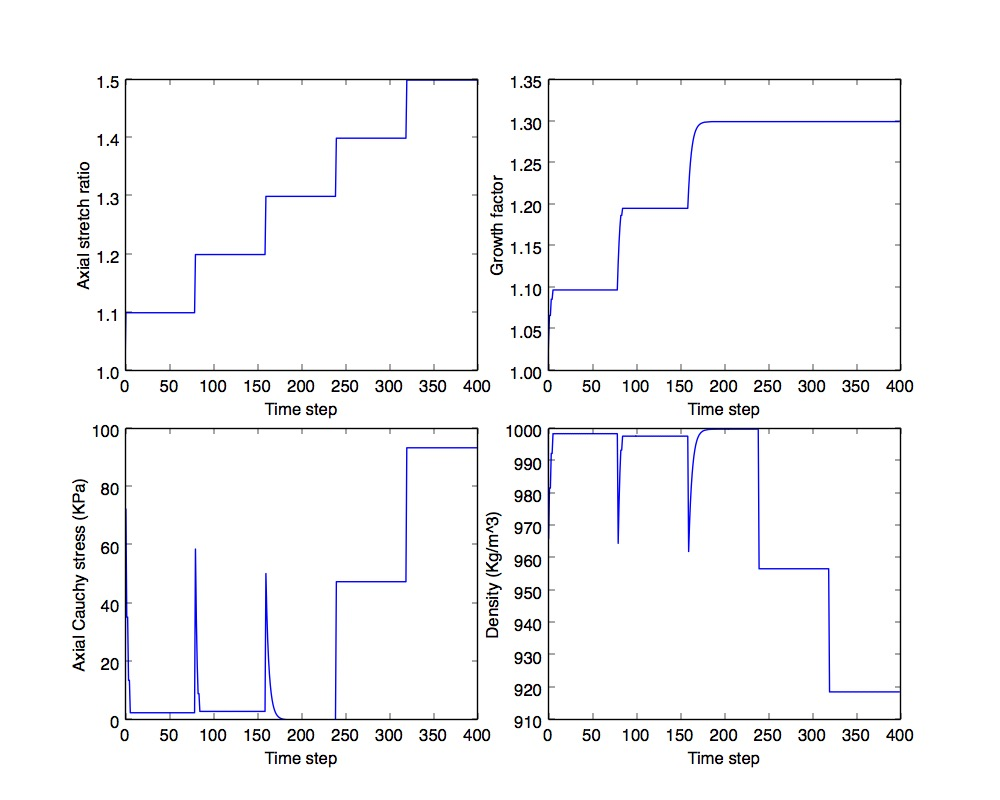
\includegraphics[width=0.8\textwidth]{./figs/stretch.jpg}
	\label{fig:uniaxial}
	\caption{Uniaxial stretching test with growth. The stretch is applied steppedly. The stress and density always recover to the initial values before the maximum growth factor is reached, which is known as biological equilibrium.}
	\label{fig:growth_results}
\end{figure}

\begin{figure}[H]
	\centering
	\begin{subfigure}
		\centering
		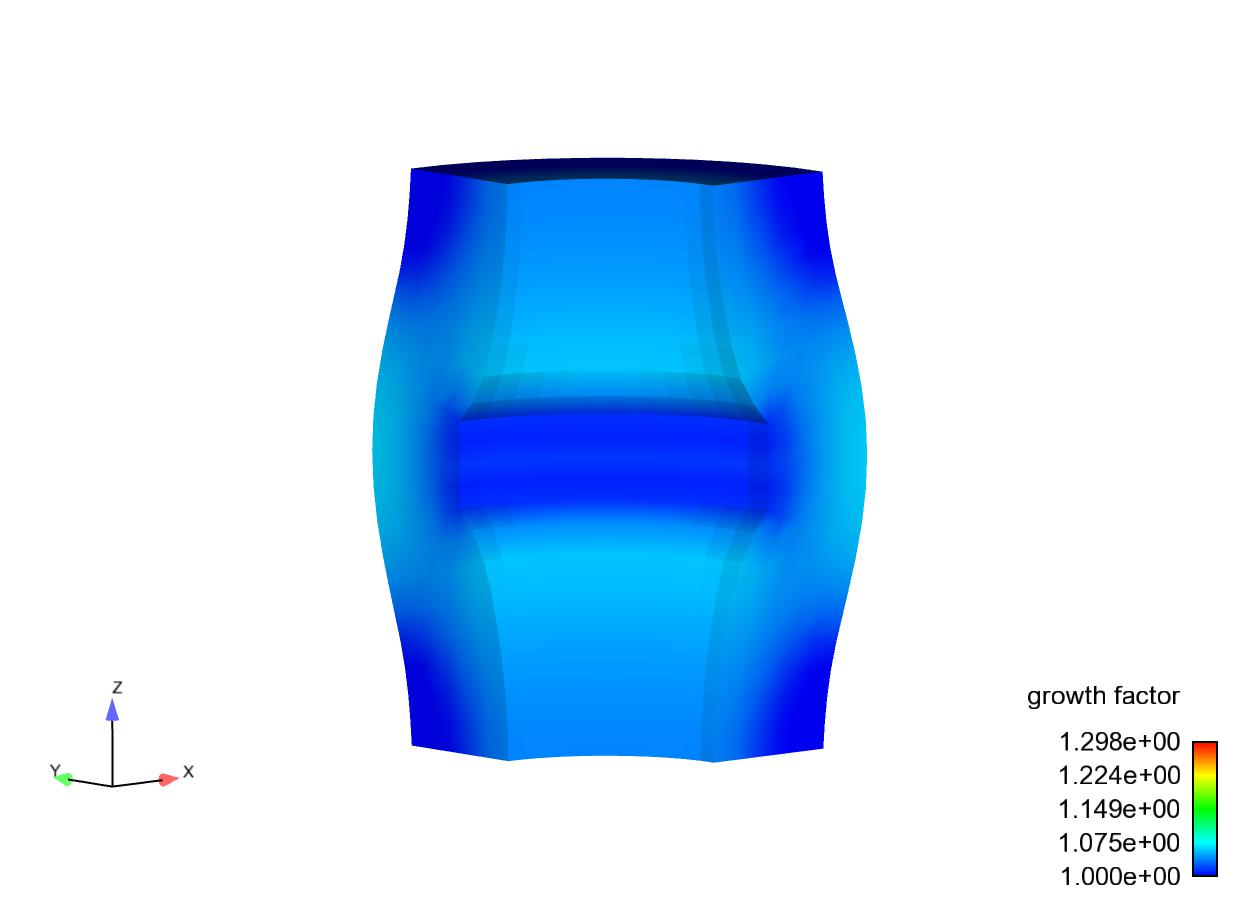
\includegraphics[width=0.3\textwidth, height=0.3\textheight]{./figs/step1.jpg}
		\label{fig:step1}
	\end{subfigure}
	\begin{subfigure}
		\centering
		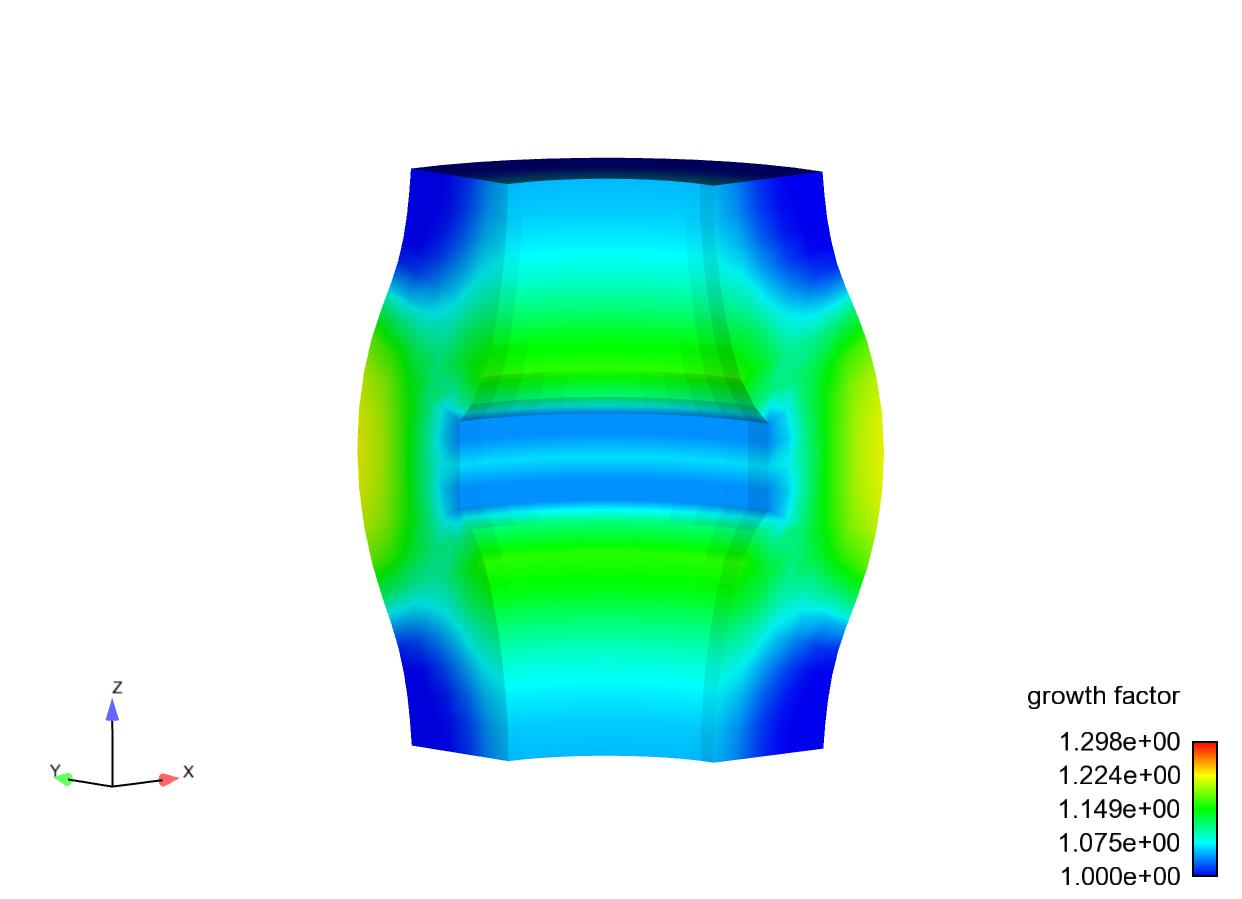
\includegraphics[width=0.3\textwidth, height=0.3\textheight]{./figs/step5.jpg}
		\label{fig:step5}
	\end{subfigure}
	\begin{subfigure}
		\centering
		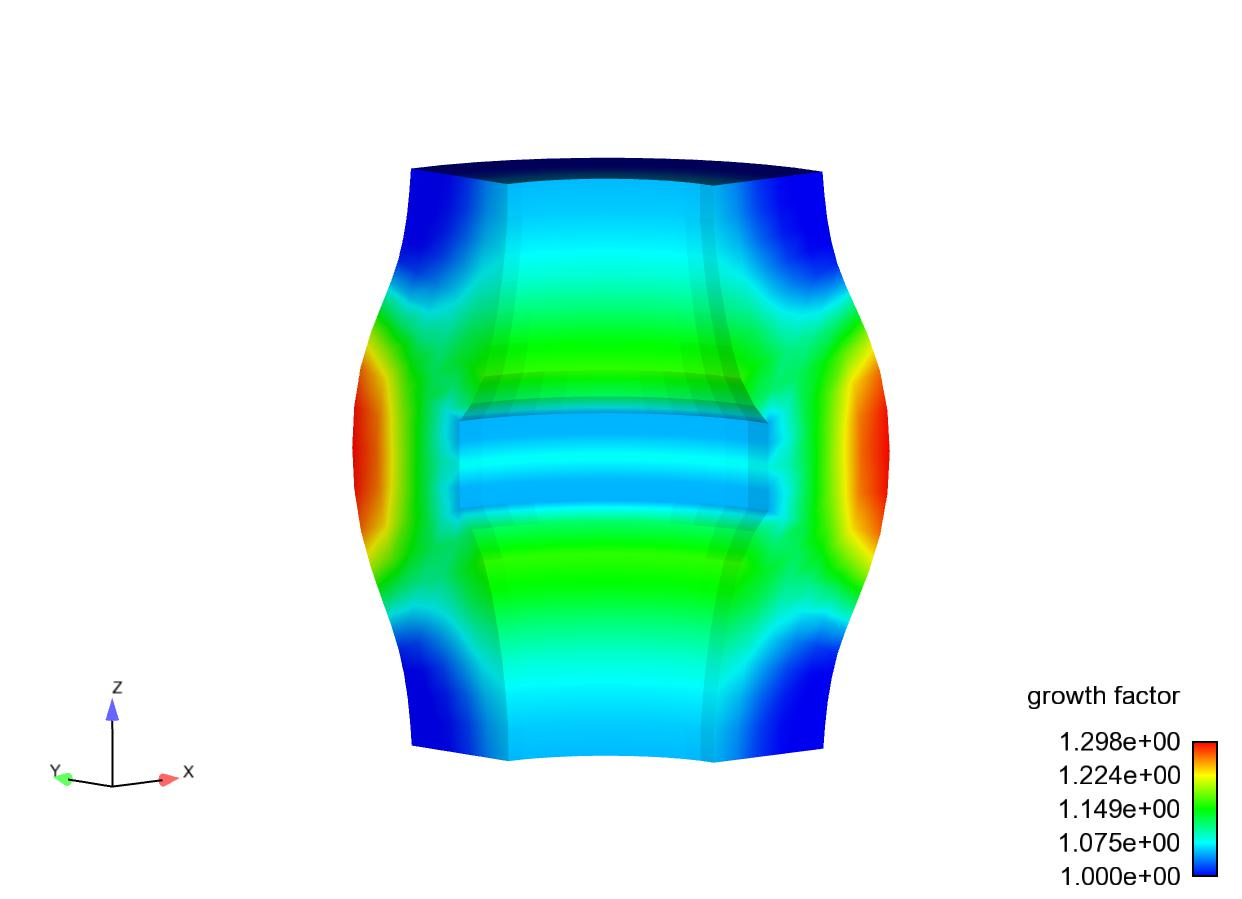
\includegraphics[width=0.3\textwidth, height=0.3\textheight]{./figs/step15.jpg}
		\label{fig:step15}
	\end{subfigure}
	\caption{(a) beginning of the growth (b) during the growth (c) after the growth}
	\label{fig:growth_stent}
\end{figure}

\section{PROPOSED WORK - 6 pages}

\subsection{Task 1: Growth Models}
\subsubsection{Multiplicative decomposition and density transformation}
The key idea of the kinematics of the growth model is the multiplicative decomposition of deformation gradient $\bF$ into an elastic part $\bF_\rme$ and a growth part $\bF_\rmg$. Based on the work in \cite{Himpel, Goktepe2}, an intermediate configuration $B_\rmg$ is introduced between the reference configuration $B_0$ and the current configuration $B_\rmt$. As shown in Figure \ref{fig:decomposition},
$\phi$ is the mapping from $B_0$ to $B_\rmt$, and the deformation gradient $\bF$ is defined in regular way as $\bF = \nabla_\bX \phi$. We assume there exists a decomposition:
\begin{equation} \label{eq:decomposition}
\bF = \bF_\rme \cdot \bF_\rmg
\end{equation}

\begin{figure}[H]
	\centering
	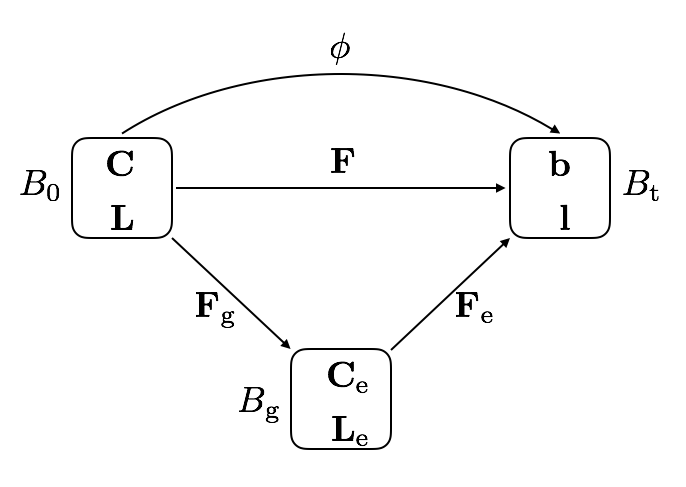
\includegraphics[width=0.45\textwidth]{./figs/decomposition.png}
	\caption{The intermediate configuration and the decomposition of deformation gradient}
	\label{fig:decomposition}
\end{figure}

Similarly, the right Cauchy-Green tensor $\bC$, velocity gradient $\bl$, Piola-Kirchhoff stress $\bold{P}$ and the second Piola-Kirchhoff (PK2) stress $\bS$ can be decomposed into elastic and growth parts as well.  Because of the growth of mass, the mapping $\phi$ is ``one-to-one'', but not ``onto''. Therefore the intermediate configuration is incompatible \cite{Cowin}.

Next we consider the density expressions in different configurations, which is the basis of the balance equations. Let $\rho_0$ denote the density in the reference configuration, $\rho_\rmt$ and $\rho_\rmg$ denote its counterparts in the spatial configuration and the intermediate configuration, respectively. Similarly, define the volume of a material particle in the reference,  spatial and intermediate configurations as $dV$, $dv$ and $dV_\rmg$, respectively. In analogy to $J = \mathrm{det}\bF$, define the Jacobians $J_\rme = \mathrm{det}\bFe$ and $J_\rmg = \mathrm{det}\bFg$. The transformations of the volumes become:
\begin{equation} \label{eq:volume}
dv = JdV, \quad dV_\rmg = J_\rmg dV, \quad dv = J_\rme dV_\rmg
\end{equation}
and
\begin{equation} \label{eq:det}
J = J_\rme J_\rmg
\end{equation}

Based on the definitions, we have the following density transformations:
\begin{equation} \label{eq:mass}
\rho_\rmg dV_\rmg = \rho_\rmt dv, \quad \rho_\rmg = J_\rme\rho_\rmt
\end{equation}

\subsubsection{Balance laws}
The local form of the balance of mass balances the rate of change of the grown density ${\bar{\rho}}_0$ with 
a possible mass flux $\bold{R}$ and a possible mass source $R_0$,
\begin{equation}
\dot{\bar{\rho}}_0 = \nabla_\bold{X} \cdot \bold{R} + R_0
\end{equation}
where the grown density is defined in the reference configuration and can be expressed as $\grho = J\rho_\rmt = J_\rmg \rho_\rmg$. From a microscopic point of view, the mass flux can be related with cell migration and the mass source can be associated to cell proliferation, hyperplasia, hypertrophy, mitosis, necrosis, and apoptosis \cite{Menzel}.

The linear momentum balance, compared to the original form, contains an additional term due to the density change:
\begin{equation} \label{eq:momentum}
\dot{\bar{\rho}}_0 \bv + {\bar{\rho}}_0\dot{\bv} = \nabla_\bX \cdot \bold{P} + {\bar{\rho}}_0\bold{b}
\end{equation}

The balance of entropy is built on the assumption that the temperature $\theta$ remains constant, which is reasonable for living biological tissues. The local form of the dissipation inequality is written as:
\begin{equation} \label{eq:entropy}
\grho \mathcal{D}= \bold{P} : \dot{\bF} - \grho \dot \Psi  - \theta(\nabla_\bX \cdot \bS - S_0) \geq 0
\end{equation}
where $\Psi$ is the free energy per unit mass and $\bS$ and $S_0$ are the extra entropy flux and source that are necessary to satisfy the second law of thermodynamics.

\subsubsection{Constitutive equations of growth}
In general, the constitutive equations for finite growth consists of three components: (i) the definition of the stress, which can be derived as conjugate counterpart of the deformation tensors; (ii) the definition of the growth tensor $\bF_\rmg$, which can be either compressible or incompressible, either isotropic or anisotropic, based on the microstructure of the modeling object; (iii) the definition of a internal variable to evaluate the growth process and a set of evolution equations to characterize it. Assume an isotropic hyperelastic model with the Helmholtz free energy $\phi(\bC, \bF_\rmg)$ (an extension to anisotropic hyperelastic model is straightforward, but is not of our interest in this project), the PK2 stress and Kirchhoff stress can be evaluated as:
\begin{subequations} \label{eq:stress}
\begin{equation}
\bS = 2\frac{\partial \Psi}{\partial \bC} = 2\frac{\partial \Psi}{\partial \bC_\rme} : \frac{\partial \bC_\rme}{\partial \bC} = \bF_{\rmg}^{-1} \cdot \bS_\rme \cdot \bF_\rmg^{-T}
\end{equation}
\begin{equation}
\boldsymbol{\tau} = \bF \cdot \bS \cdot \bF^T = \bF_\rme \cdot \bS_\rme \cdot \bF_\rme^T
\end{equation}
\end{subequations}
where $\bS_\rme$ denotes the elastic part of $\bS$. The constitutive moduli $\bold{L}$ and $\bold{e}$ read:
\begin{subequations} \label{eq:moduli}
\begin{equation}
\bold{L} = 2\frac{d\bS(\bF, \bF_\rmg)}{d\bC}
\end{equation}
\begin{equation}
\bold{e} = (\bF \overline\otimes \bF) : \bL : (\bF^T \overline\otimes \bF^T)
\end{equation}
\end{subequations}
It can be seem immediately from Equations \ref{eq:stress} and \ref{eq:moduli} that both the stress and its constitutive modulus differ from their usual form only by an additional variable $\bF_\rmg$, which is determined independently by the governing equations of the growth. Again, this resembles the concept of finite growth resembles finite strain plasticity in the sense that the basic constitutive equations themselves remain unchanged, however, they are evaluated exclusively in terms of the kinematic quantities of the intermediate configuration.

The growth deformation tensor $\bF_\rmg$ can be either isotropic or anisotropic, considering the orthotropic nature of biological tissues, the general format of $\bF_\rmg$ is written as:
\begin{equation}
\bF_\rmg = \theta_\rmf \bold{f}_0 \otimes \bold{f}_0 + \theta_\rms  \bs_0 \otimes \bs_0  + \theta_\rmn  \bn_0 \otimes \bn_0
\end{equation}
where $\bold{f}_0$, $\bs_0$, and $\bn_0$ are the unit vectors of the orthotropic microstructure in the reference configuration and $\boldsymbol\theta_\rmg = [\theta_f, \theta_s, \theta_n]$ denotes the set of internal variables which are often referred to as growth multipliers. The growth multipliers are $1$ in the plain elastic deformation, are greater than $1$ in growth and smaller than $1$ in atrophy. To model the evolution of the growth multipliers, the rate of growth multipliers are usually specified as:
\begin{equation} \label{eq:stretchRatio}
\dot{\boldsymbol\theta_\rmg} = \bold k_\rmg(\boldsymbol\theta_\rmg) \cdot \boldsymbol \phi_\rmg(\bF_\rme)
\end{equation}
where the $\boldsymbol\phi_\rmg$ is a growth criteria function to enforce a threshold on the growth, $\bold k_\rmg$ is a weighted function to prevent the unlimited growth.

\subsubsection{Mass source and mass flux}
Finally, to complete the growth model, either mass source $R_0$ or mass flux $\bold{R}$ needs to be specified. In general, the mass source $R_0$ is a scalar-valued tensor function of the state variables, their material time derivatives, and additional arguments to be specified. It may take different specific forms. For soft tissues, it is typically assumed that the density remains constant upon growth, which means $\rho_\rmg = \mathrm{const}$ and $\dot\rho_\rmg = 0$. In this case, the mass source will be evaluated as $R_0 = \bar{\rho}_0\mathrm{tr}\bL_\rmg$, where $\bL_\rmg$ is the growth part of velocity gradient, and can be easily determined by the growth tensor $\bF_\rmg$. Hard tissues, on the other hand, are characterized through an energy-driven evolution of the density, and the mass source $R_0$ is specified in terms of the grown density in reference configuration ${\bar\rho}_0$ and the free energy $\Psi$ as $R_0 = \kappa_\rho[ ( {\bar\rho}_0/{\rho_0^*} )^{-m}\Psi_0 - \Psi_0^* ]$, where $m$ is an additional parameter to ensure numerical stablility and $\kappa_\rho$ is a constant, and $\rho_0^*$ and $\Psi_0^*$ are the reference value of density and free energy, respectively.

There are two types of forms of mass flux: gradient-based flow for volume growth and surface-based flow for surface growth. In this project we adopt the first type as our main concern is the volume growth. In analogy to Fourier's law of heat conduction, the mass flux can be written as $\bold{R} = \bold{D} \cdot \nabla_\bX {\bar\rho}_0$, where $\bold{D}$ is the symmetric conductivity tensor which maps the gradient of the referential mass density ${\bar{\rho}}_0$ onto the mass flux $\bold{R}$.










\subsection{Task 2: Numerical Framework of Growth Models in Fluid Environment}
The numerical framework in this project is novel as the existing models are quasi-static such that the velocity and acceleration are assumed to be $0$ in the momentum equation, therefore the left-hand side of Equation \ref{eq:momentum} becomes $\bold{0}$. Although this assumption is reasonable because the solid growth happens very slowly, it also fails to reflect the fact that the growth is immersed in fluid environment and the solid deformation is constantly disturbed by fluid flow. In our model, a disturbance will be given as the initial velocity of the fluid field, which will enforce a non-zero essential boundary condition on the solid tissue. 

\subsubsection{Fluid governing equations with mass flux}
Because of the mass transfer at the fluid-solid boundary, the mass equation needs to be modified. Recall the mass conservation of incompressible fluid states that the mass rate per unit volume is $0$, considering the mass flux, it is rewritten as:
\begin{equation}
\rho \nabla \cdot \bv = \nabla \cdot \bold{r}
\end{equation}
%\begin{equation}
%\rho \frac{D\bv}{Dt} = -\nabla p + \mu \nabla^2 \bv
%\end{equation}
where $\bold{r}$ is the mass flux in the current configuration. 

Let us also exam the momentum equation. In our IFEM formulation, the fluid mesh is fixed. The existence of the solid is detected by the ``artificial fluid". As the solid increases in volume, the artificial fluid will also increase in volume, which automatically takes care of the real fluid momentum on its own. Therefore, the momentum equation remains unchanged.

\subsubsection{Implementation}
Two improvements proposed are the mechanical stimulus from the fluid and the mass transfer from the fluid to the solid. Towards these ends, the overall framework must appropriately address these issues: (1) through the coupling of fluid and solid simulation, correctly identifying the mechanical stimuli applied to the solid growth, including both pressure and shear stress; (2) proposing reasonable assumptions on the mass flux, which is another essential impact on the growth process.

Figure \ref{fig:framework} represents the overall framework. It can be seen that the solid growth is fully coupled with fluid environment. Following our previous work in \cite{Zhang, Zhang3, Zhang16, Zhang17}, the fluid and solid are solved individually on different meshes. The interface velocity is distributed from the fluid to the solid and the volume force is distributed from the solid to the fluid. An initial disturbance is applied to the fluid, which is the only input to the coupled growth system except for the mass source.
\begin{figure}[H]
   \centering
   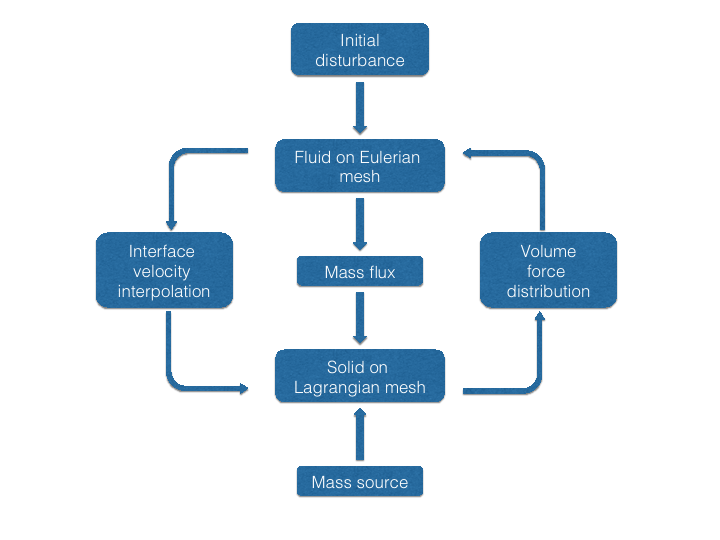
\includegraphics[width=.5\textwidth]{./figs/framework.png} % requires the graphicx package
   \caption{The numerical framework}
   \label{fig:framework}
\end{figure}







\subsection{Task 3: Mutli-time Scale in Growth Models}
In the coupled growth modeling, two key processes: the cardiac cycle and the tissue growth have very different time scales. A cardiac cycle is short, during which the blood flow oscillates drastically. Tissue growth, on the other hand, happens very slowly. If a large time step is adopted, the transient behavior of the blood flow will not be captured, thus the mechanical stimulus on the tissue can not be identified; if a small time step is used, simulating the coupled growth will be too computational expensive. Inspired by Humphrey's work in theory of mixture \cite{Baek}, we will introduce the theory of small on large to the continuum approach of growth modeling.

The theory of small on large is an idea to impose a computational process with small characteristic time to a process with large characteristic time. In our method, the cardiac cycle and the growth are computed alternately with different time steps. In order to identify the mechanical stimulus, which causes the tissue growth, we use small time step. Since the growth period is much longer than a cardiac cycle and the changing in shape occurs in a cardiac cycle is negligible, we assume the growth is ``frozen". Based on the ``frozen" configuration of tissue, the transient pressure and wall shear stress applied to the tissue are calculated. After the simulation of cardiac cycle is finished, the coupled growth will be computed alternately. The mechanical load will be calculated from the profiles of pressure and wall shear stress by evaluating the time-average values. At this step, the coupled growth will be solved with the presence of mass flux as well as a disturbed fluid field. Thus a closed loop which uses two different time scales separately is formed.

Denote the current and next time steps of in the growth model as $t_\mathrm{n}$ and $t_\mathrm{n+1}$. Take a long, straight vessel as an example, the process of the theory of small on large can be illustrated as Figure \ref{fig:smallOnLarge}:
\begin{figure}[H]
   \centering
   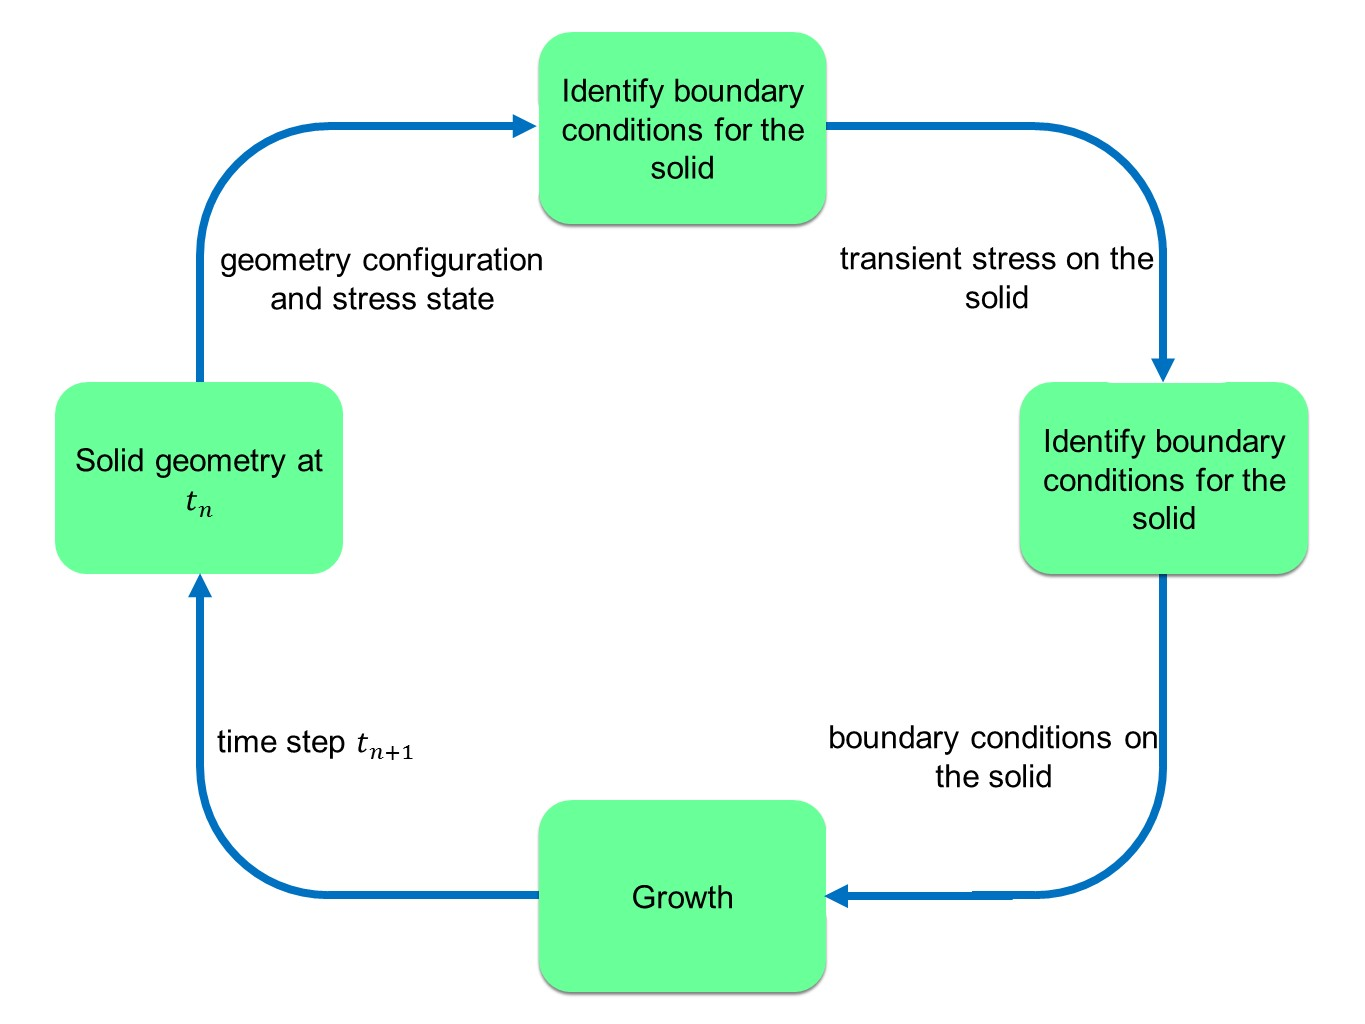
\includegraphics[width=.4\textwidth]{./figs/smallOnLarge.jpg} % requires the graphicx package
   \caption{Iteration and the information passing in the theory of small on large}
   \label{fig:smallOnLarge}
\end{figure}

The effect of the fluid on the solid is classified as the hydrostatic pressure $p(\bold{X})$ and wall shear stress ${\boldsymbol{\tau}}(\bold{X})$ which are functions of the undeformed coordinates $\bold{X}$. Let $T$ be the computational period of the FSI process, the average pressure $\bar{p}(\bold{X})$ and wall shear stress $\bar{\boldsymbol{\tau}}(\bold{X})$ can be obtained as:
\begin{subequations}
\begin{align}
\bar{p}(\bold{X}) &= \frac{1}{T}\int_0^T p(\bold{X}) dt\\
\bar{\boldsymbol{\tau}}(\bold{X}) &= \frac{1}{T}\int_0^T \boldsymbol{\tau}(\bold{X}) dt
\end{align}
\end{subequations}

\section{BROADER IMPACT - 3 pages}

\subsection{Technical Impact}

\subsection{Outreach Activities}


\section{QUALIFICATIONS OF PARTICIPANTS - 0.5 page}

\section{PROJECT MANAGEMENT \& TIMELINE - 1 page}
\section{RESULTS FROM PRIOR NSF SUPPORTS - 0.5 page}
%
%Dr. Zhang, as a co-PI, recently completed a NSF grant, ACI-1126125, entitled ``MRI: Acquisition of a Balanced Environment for Simulation'', 9/1/2011-8/31/2015 (PI: Christopher Carothers), with a total funded amount of \$2,657,633. 
%The goal for this MRI (major research instrument) award was the construction of the compute core of the cyberinstrument Blue Gene/Q. 
%%
%\textbf{Intellectual Merit}: This project supported building a powerful MRI cyberinstrument combining IBM's new Blue Gene/Q system with integrated large-scale high-performance storage and visualization components 
%that provided 
%a balanced computation and data storage cyberinstrument for massively parallel simulations and data analytics. 
%%
%\textbf{Broader Impacts}: This cyberinstrument provided a new major research capability that is now accessible to a diverse set of disciplinary and inter-disciplinary researchers, students and industry collaborators. The instrument's combination of scale, balance, and Internet accessibility made it particularly valuable for under-served researchers, such as those from states and minority-serving institutions who would not otherwise have access to such a powerful resource.
%%
%Fourteen articles were published from Dr. Zhang using the equipment built with the grant \cite{li-particletransport-2015,cwang2013,wang-zhang-mifem,zhang2013,zhang2014,chuwang2015,wang2012semi,wang2013modified,zhang2013advancements,yong-2013-jcp,yong2013,yong-slip2013,chuwang2014,zhang2014modeling}, while 2 are under review \cite{yang2016VFdraft,yang2016PMLdraft}. Research product from this grant also includes established open-source software tools to study biomedical applications involving fluid-structure interactions, currently published and maintained on Github. 
%
\clearpage
\pagenumbering{arabic}
%\bibliography{cancer-refs,zhang2013-2016,refs-lucy,fem,chuthesis,Cell_NP,porous}
\bibliographystyle{unsrt}
\bibliography{references}
\end{document}
